\documentclass[12pt]{article}
\usepackage[utf8]{inputenc}
\usepackage{graphicx}

\title{Master's thesis proposal}
\author{Cristian Manuel Abrante Dorta}
\date{July 2021}

\begin{document}

\maketitle

\section{Introduction}

During recent years there has been some discussions about how to correctly organize and deploy service oriented architectures. One of the software architecture patterns that has gained more popularity nowadays are microservices. Many big, mid-level and even small software companies had adopted this architecture due to its tremendous benefits in comparison with traditional and monolithical software applications. \\

Microservices are basically an extension of service oriented architecture. The main goal, is that each of those microservices offer a well-defined and clear scope of functionalities, that can be accessed by another microservice using \textit{remote procedure calls} \cite{nelson1981remote}. The main advantage of this pattern is that it can be established a clear ownership of each microservice by different teams where they are responsible for the development, maintenance and deployment of them. This presents a clear advantage in comparison to the classical \textit{monolithic} architecture, because on those, even though the development tasks could be divided in different teams, the deployment of a single functionality implies the deployment of all the system, being then prone to cause important problems that can shut down completely the application. \\

Even though microservices architecture represents an step forward in the design of software systems, it also have some drawbacks in comparison with the monolithic architectures, such as the performance. In traditional monolithic application the calls to subroutines is something that can be resolved inside the same process and machine, however in microservices, the call have to be done over the network, which is something that can eventually introduce some delays in the execution. Apart from this, there is another problem that microservices architectures have to face, which is the handling of over thousands of different microservices, when considering businesses that operates at big scale. In this case, any issue caused by one microservice, can be extended through many of them, and engineers have to debug calls that comes from a huge stack different services which is something that can be challenging and time-consuming.\\

This is why many companies had adopted the pattern of \textbf{Domain-Oriented Microservice Architecture} \cite{DOMAUber}. Using this architecture, many microservices can be grouped inside a logical division that can fit the needs of the company. Those logical divisions are called \textbf{Domains}. For isolate the domains and make easier their maintenance and debugging, one approach that many companies had applied is to create a common gateway that expose the interface (usually as routes that can be called with different HTTP methods). Apart from being the single entry point for specific domains, the gateway can also provide different high-level responsibilities, such as authentication, routing, rate limiting, load ballancing etc. This pattern had been widely adopted by companies that operate at a high level such as Uber \cite{GatewayUber}, or Unity Technologies.\\

\begin{figure}[h]
    \centering
    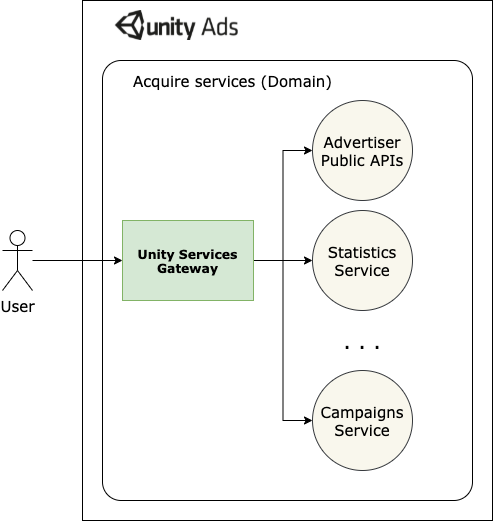
\includegraphics[scale=0.35]{src/proposal/img/unity-services-diagram.png}
    \caption{Unity Acquire microservices architecture setup}
    \label{fig:unity-services-diagram}
\end{figure}

Taking into consideration all this concepts, this thesis aim is to focus on the particular case of the Acquire division of Unity Technologies (Figure \ref{fig:unity-services-diagram}). Unity Technologies is a company based on the United States whose aim is to create tools that help developers to create games and other 3D products. It also runs UnityAds, one of the biggest advertisement networks in the world, and which is one of the main income sources that the company offers to the creators in order to run a successful business out of their games. The Acquire division contains all the tools for the publishers to create and run different advertisement campaigns in their games.\\

From the software perspective, the acquire division can be considered a domain in a Domain-Oriented Microservice Architecture. Functionalities are divided into services that are owned by different teams, and those teams are responsible for their development and deployment. Furthermore, the domain also contains a gateway (Unity services gateway) that is the entry point for all the microservices. Apart from that, it also implements some common top-level functionalities.\\

The gateway is in itself a service too, and monitoring the state of it is a crucial task for guaranteeing the good health of the overall system. In particular, one type of monitoring that is interesting to do is the logging of the errors that are produced at gateway level, such as organization or rate limiting errors. For many teams, which are responsible of services that depends on the gateway, is common to ask these type of questions: \textit{which users or organizations are hitting our rate limits?}, \textit{Which is the amount or the frequency of authentication errors that our system is having?}\\

Considering the current setup of the system, those questions are not trivial to answer. Because when an error happens at gateway level, it usually sends the corresponding response to the user but it does not register it in a way that can be easily explored and visualized afterwards. Even though the technology stack where usually those microservices are deployed have a lot of logging and visualization functionalities, for example the Google Cloud environment, usually they have some limitations when crossing information that can be interesting at visualization level (for example obtaining some data from databases that are not deployed using the same technological stack).\\ 

Taking all this into account, the objective of this thesis is to propose a method on how to correctly monitor and visualize the top-level errors that the gateway of a Domain-Oriented architecture produce, and how to visualize those errors in an effective way for allowing the communication between the involved teams.

\section{Expected outcomes}

As discussed before, the expected outcome of this thesis is an extensive research about how can the errors produced by a services gateway in the context of a Domain-Oriented architecture be properly handled. This knowledge is going to be applied to the particular case of the Unity Services Gateway, adapting to the technological stack that the company is using at the moment (Figure \ref{fig:project-outcome}).

\begin{figure}[h]
    \centering
    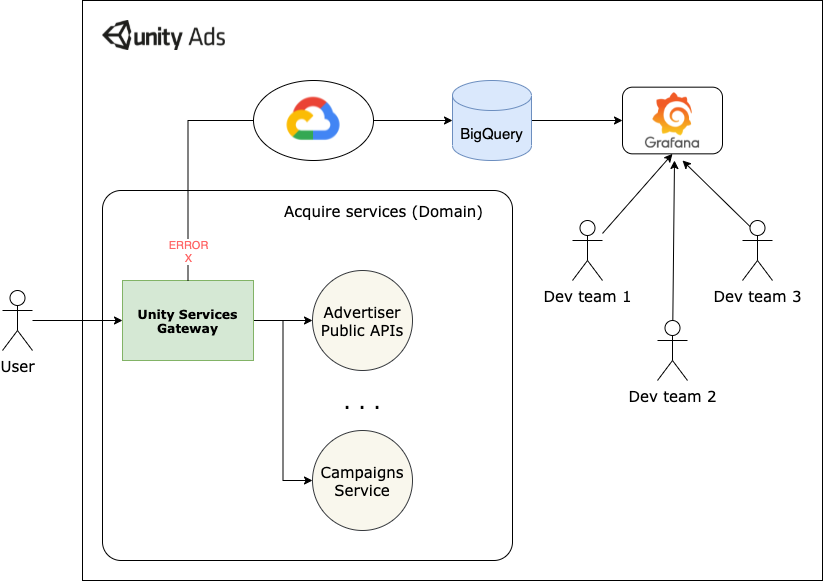
\includegraphics[scale=0.25]{src/proposal/img/Unity Services Gateway - project.png}
    \caption{Diagram representing the expected software products.}
    \label{fig:project-outcome}
\end{figure}

Taking that into consideration, the software products that are going to be produced are the following:

\begin{itemize}
    \item \textbf{Error emitter}: This software is responsible of collecting the errors produced in the Unity Services Gateway and then emit them to the log sink.
    \item \textbf{Log sink}: This software is responsible for receiving the errors and store them in the big data platform.
    \item \textbf{Big data platform}: Due to the scale and number of request of this type of systems, it is crucial to use a big data platform in order to store the information. The chosen plattform is going to be BigQuery as it is easy to integrate with the current setup of the company.
    \item \textbf{Visualization tool}: As the communication is an important purpose of this project, one of the main software products that is going to be produced is the visualization tool for the errors that are emitted.
\end{itemize}

For the execution of this project, the following steps are going to be followed:\\

\begin{enumerate}
    \item Research the state of the art in microservices architecture monitoring, focusing on the case of a service that is receiving thousands of simultaneous requests.
    \item Define the structure of the events that are going to be emitted. Decide which fields are useful for being stored.
    \item Create the tables in the Big Data platform in order to match the events previously decided.
    \item Implement the event emitter on the services gateway.
    \item Implement all the log sink synchronization.
    \item Create the visualization tool.
\end{enumerate}

It is important to remark that some steps might be considered an iterative process, especially the creation of the visualization tool, as some feedback might be collected from different teams in order to improve the resulting software product.

\bibliographystyle{plain}
\bibliography{proposal}

\end{document}
